\documentclass[a4paper]{article}

%% Language and font encodings
\usepackage[english]{babel}
\usepackage[utf8x]{inputenc}
\usepackage[T1]{fontenc}
\usepackage{relsize}
\usepackage{xcolor}

%% Sets page size and margins
\usepackage[a4paper,top=3cm,bottom=2cm,left=3cm,right=3cm,marginparwidth=1.75cm]{geometry}

%% Useful packages
\usepackage{amsmath}
\usepackage{graphicx}
\usepackage{amssymb}
\usepackage[colorinlistoftodos]{todonotes}
\usepackage[colorlinks=true, allcolors=blue]{hyperref}

\usepackage[lf]{Baskervaldx} % lining figures
\usepackage[bigdelims,vvarbb]{newtxmath} % math italic letters from Nimbus Roman
\usepackage[cal=boondoxo]{mathalfa} % mathcal from STIX, unslanted a bit
\renewcommand*\oldstylenums[1]{\textosf{#1}}

\title{Robustified RG, MIMO System}
\author{You}

\begin{document}
\maketitle

\begin{abstract}
Your abstract.
\end{abstract}

\section{Introduction}

Dealing with a mass-spring-damper MIMO system with 2 inputs (Forces) and 2 outputs(Positions).
First, we perform experiments to do a MIMO-ARX identification of the system. Then, 2 separate dynamic models are extracted, one nominal and the other that generates the output error. This model that generates the output error is the disturbance model used to capture model uncertainty. Zero-measurement noise assumption is made.

\section{Identification}
Experiments are performed with the following parameters: \\
\begin{equation}
\begin{matrix}
\begin{matrix}
	dt = 0.1s \\
	N = 10000 \\
	u_1 = 1000*randn(1,N) \\
	u_2 = 1000*randn(1,N) \\
	\alpha = 0.05
\end{matrix}
&
\begin{matrix}
na = \begin{bmatrix}2 & 1 \\ 1& 2 \end{bmatrix} \\
nb = \begin{bmatrix}2 & 2 \\ 2& 2 \end{bmatrix} \\
nk = \begin{bmatrix}1 & 0 \\ 0& 1 \end{bmatrix} \\
\end{matrix}
\end{matrix}
\end{equation}
\hspace{80pt}
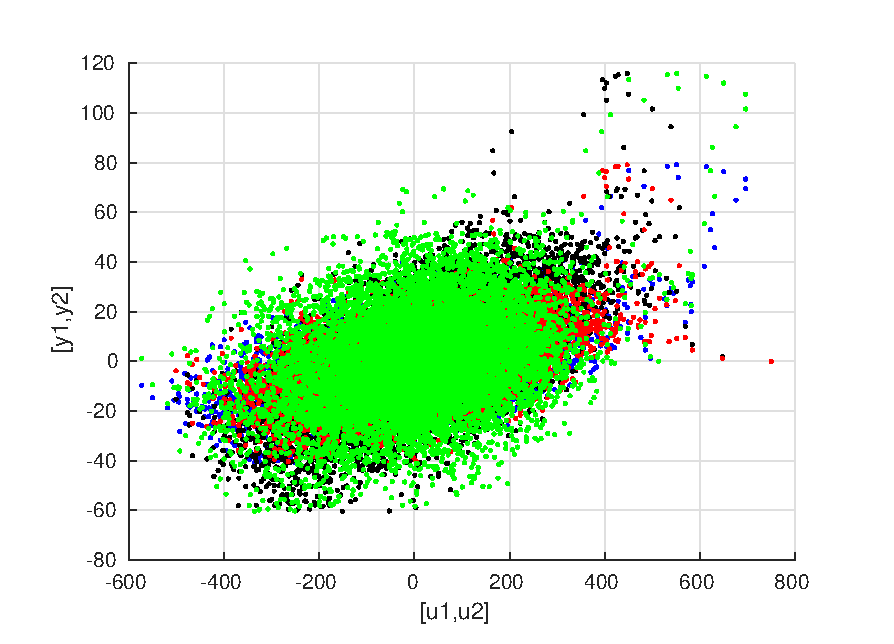
\includegraphics[scale=0.6]{Figures/id_data.eps} \\
Using the ARX identification toolbox from MATLAB, the following I/O model is identified
\begin{equation}
\begin{bmatrix}
A_{11}(z^{-1}) & A_{12}(z^{-1}) \\
A_{21}(z^{-1}) & A_{22}(z^{-1})
\end{bmatrix}
\begin{bmatrix}
y_1(t) \\ y_2(t)
\end{bmatrix} = 
\begin{bmatrix}
B_{11}(z^{-1}) & B_{12}(z^{-1}) \\
B_{21}(z^{-1}) & B_{22}(z^{-1})
\end{bmatrix}
\begin{bmatrix}
u_1(t) \\ u_2(t)
\end{bmatrix} +
\begin{bmatrix}
1 & 0 \\ 0 & 1
\end{bmatrix}
\begin{bmatrix}
w_1(t) \\ w_2(t)
\end{bmatrix}
\end{equation}
Rewriting this as $\textbf{A}y(t) = \textbf{B}u(t)+\textbf{C}w(t)$ and inverting \textbf{A}, we get $y(t) = \textbf{A}^{-1}\textbf{B}u(t) + \textbf{A}^{-1}\textbf{C}w(t)$. This leads to two models with inputs $u(t)$ and $w(t)$, the sum of whose outputs captures all the dynamics of the system. It is made sure that the resultant systems are stable.
\\ \\
Converting the models $\Sigma_M:y_M(t) = \textbf{A}^{-1}\textbf{B}u(t)$ and $\Sigma_D:e(t) = \textbf{A}^{-1}\textbf{C}w(t)$ into state-space models and adding the outputs, we get the complete system as:
\begin{equation}
\begin{matrix}
\begin{bmatrix}
x_M(k+1) \\ x_D(k+1)
\end{bmatrix}
=
\begin{bmatrix}
A_M & 0 \\
0 & A_D
\end{bmatrix}
\begin{bmatrix}
x_M(k) \\ x_D(k)
\end{bmatrix}
+
\begin{bmatrix}
B_M \\ 0
\end{bmatrix}u(k)
+
\begin{bmatrix}
0 \\ B_D
\end{bmatrix}w(k) \\ \\
y(k) = 
\begin{bmatrix}
C_M & C_D
\end{bmatrix}
\begin{bmatrix}
x_M(k) \\ x_D(k)
\end{bmatrix}
+
\begin{bmatrix}
D_M 
\end{bmatrix}u(k)
+
\begin{bmatrix}
 D_D
\end{bmatrix}w(k) \\ \\
x_M \in \mathbb{R}^{n_M}, x_D \in \mathbb{R}^{n_D}
\end{matrix}
\end{equation}
It is noted that since there is the assumption of zero-measurement noise, the control algorithm designed which used this models has to regulate the actual output $y(k)$, which includes the additive disturbance. 
\section{State estimator}
Following the identification, a state estimator is designed to estimate the states $x_D(k)$ of the disturbance model. This is because the signal $w(k)$ is unknown. An optimal estimator $L_D$ is designed, which updates the states according to the following equations:
\begin{equation}
\begin{matrix}
\begin{bmatrix}
\hat{x}_M(k+1) \\ \hat{x}_D(k+1)
\end{bmatrix}
=
\begin{bmatrix}
A_M & 0 \\
0 & A_D
\end{bmatrix}
\begin{bmatrix}
\hat{x}_M(k) \\ \hat{x}_D(k)
\end{bmatrix}
+
\begin{bmatrix}
B_M \\ 0
\end{bmatrix}u(k)
+
\begin{bmatrix}
0 \\ L_D
\end{bmatrix}(y(k)-\hat{y}(k)) \\ \\
\hat{y}(k) = 
\begin{bmatrix}
C_M & C_D
\end{bmatrix}
\begin{bmatrix}
\hat{x}_M(k) \\ \hat{x}_D(k)
\end{bmatrix}
+
\begin{bmatrix}
D_M 
\end{bmatrix}u(k)
\end{matrix}
\label{estimator_model}
\end{equation}
This results in error-dynamics between the actual and estimated system to evolve according to:
\begin{equation}
\begin{matrix}
\begin{bmatrix}
e_M(k+1) \\ e_D(k+1)
\end{bmatrix}
=
\begin{bmatrix}
A_M & 0 \\
-L_DC_M & A_D-L_DC_D
\end{bmatrix}
\begin{bmatrix}
e_M(k) \\ e_D(k)
\end{bmatrix}
+
\begin{bmatrix}
0 \\ B_D-L_DD_D
\end{bmatrix}w(k)\\ \\
e_y(k) = 
\begin{bmatrix}
C_M & C_D
\end{bmatrix}
\begin{bmatrix}
e_M(k) \\ e_D(k)
\end{bmatrix}
+
\begin{bmatrix}
D_D
\end{bmatrix}w(k)
\end{matrix}
\label{estimator_error}
\end{equation}
In simplified notation, this is written as:
\begin{equation}
\begin{matrix}
e_x(k+1) = A_Le_x(k)+B_Lw(k) \\
e_y(k) = C_Le_x(k)+D_Lw(k) 
\end{matrix}
\end{equation}
\section{Bound estimation}
With the $u(k)$ and $y(k)$ signals used for identification, the estimator model \eqref{estimator_model} is simulated. The difference between the actual output and estimated output is captured as the signal $e_y(k)$, which is the output of the system \eqref{estimator_error}. The input signal $w(k)$ to this system is unknown. \\
 To design a robust controller, we intend to find the smallest set in which $w(k)$ lies. For this, we construct the set $\hat{E}_\infty$ defined as $\hat{E}_\infty = \{e_y: He_y \leq h \}$, which is a polyhedral box containing all the $e_y(k)$ vectors obtained from the identification and simulation. Using $\hat{E}_\infty$, we construct a set $\hat{W}_\infty$ which satisfies:
 \begin{equation}
 \begin{matrix}
 \hat{W}_\infty = \{ w: \hat{e}_y(k|e_x,w) \in \hat{E}_\infty \hspace{10pt} \forall e_x \in \mathbb{R}^{n_M+n_D}, k \in \mathbb{N} \}\\ \vspace{-10pt} \\
 \text{where} \hspace{10pt}
 \hat{e}_y(k|e_x,w)= C_LA_L^{k-1}e_x+C_L\mathlarger{\sum}\limits_{t=1}^{k-1}A_L^{t-1}B_Lw+D_Lw
 \end{matrix}
 \end{equation}
This set can be proven to be \textcolor{red}{positive invariant}, meaning that if $w(k) \in \hat{W}_{\infty}$ is applied to the system when $e_y(k) \in \hat{E}_{\infty}$, it will lead to $e_y(k+1) \in \hat{E}_{\infty}$. For a particular value of future time instant $k$, the set $\hat{W}_{k}$ is defined as:
\begin{equation}
\hat{W}_k = \{w: \hat{e}_y(t|e_x,w) \in \hat{E}_{\infty} \hspace{10pt} \forall e_x \in \mathbb{R}^{n_M+n_D}, t \leq k, t \in \mathbb{N} \}
\end{equation}\\
To calculate $\hat{W}_{\infty}$, one can calculate $\hat{W}_k$ for increasing values of $k$ and an \textcolor{red}{arbitrary} initial condition $e_x$. Following the \textcolor{red}{finite termination} property, the sets $\hat{W}_{k}$ converge to $\hat{W}_{\infty}$. This is given by:
\begin{equation}
\begin{matrix}
\text{For increasing values of $k$:} &
\begin{matrix}
H\hat{e}_y(k) \leq h \\
H\text{\large{(}}C_LA_L^{k-1}e_x+C_L\mathlarger{\sum}\limits_{t=1}^{k-1}A_L^{t-1}B_Lw+D_Lw\text{\large{)}} \leq h \\
H\text{\large{(}}C_L\mathlarger{\sum}\limits_{t=1}^{k-1}A_L^{t-1}B_Lw+D_L\text{\large{)}}w \leq h-C_LA_L^{k-1}e_x \\
G(k)w \leq h-C_LA_L^{k-1}e_x
\end{matrix}
\end{matrix}
\end{equation}
\textcolor{red}{For a stable estimator design, $A_L$ is stable, and hence $C_LA_L^{k-1}e_x \rightarrow 0$ as $k \rightarrow 0$. Also, the finite termination property of $G(k)$ follows}.

\section{Reference governor design}
Since $w(k)$ is the model uncertainty and not noise, the controller should control the signal $y(k)$, which is given by $
y(k) = \hat{y}(k)+e_y(k)$.
The complete model generating this output

\bibliographystyle{alpha}
\bibliography{sample}

\end{document}